% chapterquote command.
\newcommand{\chapterquote}[2] {
\begin{quote}
\textit{"{#1}"}

--- {#2}
\end{quote}
\vspace{12pt}
}


\documentclass[a4paper]{report}
\usepackage{graphicx}

\author{Per Andersson, Fredrik M{\"o}llerstrand}
\title{Zohmg---a large scale data store for aggregated time-series-based
data. [DRAFT]}

\begin{document}
\maketitle

\noindent {\Large \textbf{Abstract}}
\vspace{12pt}
\noindent

% TODO: use less buzzwords; focus on the problem.

This thesis describes a data store for multi-dimensional time-series-based
data. The data is aggregated over many units of measurements and across
multiple dimensions. One of these dimensions is always time.

We present a data store called Zohmg. It is built on top of HBase and uses
Hadoop to run import jobs in parallel. Zohmg stores and serves aggregates of
measurements. The measurements are extracted taken from log files or similar
sources with user-supplied code.

The data store is optimized for speed of data retrieval: one of the design
goals was to serve data at mouse-click rate and promote real-time data
exploration. As such, Zohmg stores only the summarized data, not the atomic
measurements.

Similar data stores exist: they generally use a relational database system as
their underlying data store. The novelty of our approach is to model OLAP
cubes on top of a bigtable-like data store.

The thesis is presented in three major sections: problem statement,
theoretical solution and implementation details.


\tableofcontents
\vfill
\pagebreak

\chapter{Introduction}

\section{Background}

% TODO: introduce time-series, data warehousing, mapreduce, bigtable
% TODO: why is time important? (we query for time, etc.)

Any organization will eventually want to analyze various characteristics of
its service and operations. The services can be anything from web sites to
theme park; the analysis might include characteristics such as the number of
visitors per day, or the average time a theme park guest spends queueing for a
particular ride.

Inevitably, the services and operations will generate a log for later
analysis. As the services grow in size, so will the data sets they generate.

An important property of these data sets is that they generally have a regular
structure and are broken down into records that are independent of each other.
The records can be analyzed one at a time without losing any of their meaning
and are as such very well suited for parallel analysis.

Each log record typically contains a number of fields. For example, a log of
visits to a web site might contain a timestamp, information about what country
the visitor is from and what web browser she used.

When the records in the data set have been analyzed, one can draw conclusions
about what countries generate the most traffic to the site, which web browser
is most popular in a certain country, etc. Summaries of data are generally
called aggregates. To aggregate data, for example to compute the sum of
visitors for all European countries, is a common technique for speeding up
data lookup in data stores.

The size of the data sets at last.fm is in the range of several gigabytes per
day. Some data sets are many times larger. It is our belief that this is
typical.

A single computer is not likely to be able to process that amount of data
before a new batch arrives, and for very large data sets a single computer
would simply not be able to fit the intermediate data set in its working
memory.

It is suitable to exploit the parallel nature of the records by breaking up
the data sets in pieces and to have each piece be processed on a separate
node in a large compute cluster. It is also suitable to store the data across
many storage nodes in what is called a distributed file system.


% TODO: write about how mapreduce already solves the problem of parallel
% computation, and how gfs solves the problem of distributed storage.


% introducing variables and dimensions.

Organizations measure their operations by considering many variables. When
these variables are placed in a spreadsheet, which organizations are wont to
do, the variables are set on the x and y axes. Each axis represents a logical
grouping of variables. In the example of a log file of visits to a web site
above, country of origin is one such variable. A variable is generally called
a dimension in this paper.

The International Aerodyne Corporation, a leading exporter of woodworking
nails, uses a spreadsheet to keep track of the number of nails exported to
each country every month (see figure). 

% image of a spreadsheet.
%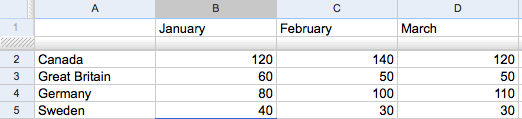
\includegraphics[width=70mm]{pictars/aerodyne-nails.png}
%\imagecaptionplease{crates of nails exported}

In the figure above, the time dimension is set on the x-axis and the country
dimension is set on the y-axis. If the Aerodyne Corporation were to start
keeping track of the kind of nails they sell (pins, tacks, spikes, etc.) in
addition to the country to which the nails were sold, they would effectively
have added a new dimension to their data.

Many organizations work with data that have more than three dimensions. Such
data is hard to manage in a spreadsheet, and the organizations need
specialized tools to analyze and visualize their data.


\section{Problem description}
% Problemsbeskrivning.

At Last.fm there is a central repository where metrics and statistics for
various services are stored. There is a web site for internal use that
displays graphs of the services and their statistics. Examples of statistics
are web site usage broken down by country, scrobbling broken down by client
and daily subscription counts.

The statistics are stored in a relational database. Each measure is stored
atomically; a summing operation across numerous rows is required to answer
queries. The database is bursting at the seams because of the size of the
data. Some of the problems with the current setup is that adding a new data
source to the database requires manual intervention and that some of the
questions that analysts ask can not be answered in real-time.

Last.fm foresees that its data sets will continue to grow and would like to
move away from the current setup towards a scalable data store. The data store
should be able to answers most questions in real time. It should be easy
to publish new data sets.


\section{Goal}
% Syftesformulering.

% TODO: define aggregates!

The goal is to build a data store that enables its users to perform
multi-dimensional analysis.

In addition, the secondary goal is to build a tool that allows users to easily
store their data sets in the data store. The tool should provide a simple – as
in minimalistic – mechanism for data analysis (import) and querying (export).

% is mapreduce part of the goal? hardly.
The data analysis will require the user to write a MapReduce map. The queries
will be performed via an export API for consumption by computer programs.

% these are more likely part of the scope.
The queries will always be made over a time range and for a single unit. The
tool will support analytical functions such as drill-down, slicing, etc.

The tool should be aware of dimensions in general and the dimension of time in
particular. Measurements will be specified in a unit. There will be no limit
on the number of units.

There should be no theoretical boundary on the number of dimensions. Common
queries must be answered expediently to allow for analysts to explore data in
real time.



\section{Scope}
% Avgransning.

% TODO: argue why we do these avgränsningar.

The data store is just that: a data store with import and export
functionality. The data store does not interpret the data it store.

The data store is time-series-based: all data must include the time dimension.

All measures are integers. Sum is the only supported aggregation function. The
data store does not support reach-like data (i.e. number of unique visitors)
since it is not summable.

There is no functionality for plotting data sets, etc.



\section{Related work}

% TODO: this section.

OLAP is something. It's drawbacks are unknown.

HDW is a system whose goal is to create a high performance large scale data
warehouse based on MapReduce and Bigtable. \cite{hdw}

Omniture is used at Last.fm etc.


\section{Overview}

This thesis describes the Zohmg system and how to use it.

% TODO: make correct.
The following overview is entirely incorrect:

Chapter 2 establish the theoretical base of the problem statement.

In chapter 3, the tools used for the implementation are declared, moving
over to chapter 4 where the details of the implementation are presented.

How to use the Zohmg system is presented in chapter~5, while chapter 6
shows an example work flow.

Chapters 7 and 8 discuss the results, related, and future work, and
presents the conclusion, respectively.



% CONCEPTS IN DATA WAREHOUSING, by clark de jean
\chapter{Concepts in Data Warehousing}

This chapter introduces data warehouses and the concept of data cubes. It then
introduces common operations on data cubes: projections, slicing and dicing,
and aggregation.


\section{Data Warehouses}

A data warehouse is a repository of an organization's electronically stored
data. Data warehouses are designed to facilitate reporting and analysis; the
core actions of a data warehouse are to load, transform and extract data.

\subsection{OLAP}

OLAP, which is an acronym for Online analytical processing, is an umbrella
term for systems built in a certain manner and that are optimized quickly
answer multi-dimensional analytical queries.

At the core of any OLAP system is the OLAP cube (also known as a
multi-dimensional cube or a hypercube). The cube consists of numeric facts
-- called measures -- which are grouped by dimensions. For example, the number
of nails sold is a measure while country, month and type of nail are
dimensions. It is from OLAP that [we] have appropriated the concept of a data
cube.


\section{Data cubes}

% looking for a mathier explanation here.
A data cube is a conceptual n-dimensional array of values. It aids in
reasoning about dimensions. In the context of this paper, each dimension of
the cube corresponds to an attribute of the data in question and each point
along the dimension's axis is a value of the corresponding attribute. At any
point where the n dimensions intersect, a measure can be found. For example,
if the dimensions are country and nail type, the point in the cube where
country is equal to Sweden and nail type is equal to tack will contain a
measurement of the units of tack nails sold in Sweden.

Data cubes are traditionally modeled as star schemas in relational database
systems. \cite{olap_solutions}


\subsection{Projections}

One of the most common operations on a data cube is the projection. A
projection is a function to another data cube, where one or more dimensions
are discarded from the cube and the measurements along each dimensions are
summed up, leaving a data cube of a lesser dimension.

For example, consider the three-dimensional data cube that represents sales of
nails; the dimensions are nail type, country and month. A projection from that
cube to one with two dimensions -- month and nail type -- would flatten the
country dimension: the measurements in the new cube represent the global sales
of each nail type for each month.


\subsection{Slice and dice}

The slice operation fixes the values of one or several dimensions in the cube.
The data omitted from this operation would be any data associated with the
values of the dimension that were not fixed. The dice operation is a slice on
more than two dimensions.

For example, consider again the three-dimensional data cube that represents
sales of nails; the dimensions are nail type, country and month. A slice of
that cube with the country dimension fixed to Germany would contains sales
figures for each nail type and month for Germany only.


\section{Aggregates}

An aggregate is a composite value that is derived from several variables.
Typical examples of aggregate functions are average, count, and sum.

For example, sales figures for a whole year may be summed up and stored along
the year dimension.

In a standard OLAP setup, a number of aggregates are pre-computed and
stored in the cube. These base aggregates represent only a fraction of the
many possible aggregations. The remaining aggregates are computed from the
base aggregates as they are demanded.

The main reason for pre-computing aggregates is to reduce access times, the
time it takes to compute an aggregate may be unacceptable to a waiting
user. Pre-computing frequently requested aggregates is therefore regularly
done in the background, giving the user fast access to these.
\cite{olap_solutions}

The classic trade-off between time and space applies to whether or not to
pre-compute an aggregate. Pre-computing too many aggregates might result in an
unfeasible amount of data, while pre-computing too few aggregates results in
longer access times for those aggregates that were not pre-computed.


\section{Summary}

This chapter introduced Data Warehouses in general and OLAP in particular. The
concept of data cubes was introduced by OLAP. The chapter was rounded off with
a discussion of dimensionality reducing operations and aggregations of data
cubes.



\chapter{System Analysis}

\chapterquote{Methods and means cannot be separated from the ultimate aim.}{Emma
Goldman}


\section*{Introduction}

This chapter will discuss and analyze the Zohmg system, that is to be built.

First the application area and the wanted system functionality are presented;
while discussing the input and output characteristics, and possible challenges.
Furthermore, a rough sketch and discussion of the Zohmg systems different
components will be presented. Secondly, the Zohmg system requirements will be
featured.

Throughout this chapter distinction is made between the developer: who develops
the application, and the user: who uses the product which the developer
creates. Although, in reality, they might be the same person.


\section{System function}

Last.fm has a central statistics and metrics tool built on a relational
database. It is possible to import analyzed data to this tool; the data is
presented to the user as graphs. Disadvantages of this system include problems
with new data source additions: they can sometimes not be loaded because they
are too big. If a user wants to perform a custom query, manual intervention by
the developer is necessary. There is no way for this system to handle custom
queries.

The data source is typically a log file; it is often a large file, up to
gigabytes in size, of structured data. The data is structured the same way on
each line, this makes writing a program for analyzing the entire data set as
simple as analyzing a single line.

Reporting the analyzed data is the final step. This is what the user is
interested in: viewing the analyzed data. The tool at Last.fm presents the user
with a dashboard that has a selection of graphs on primary metrics; it also has
a list of all available graphs. All the graphs are pre-aggregated, no support
exists for custom queries. Enabling the user to query the aggregated data---for
instance viewing the most popular web browser in a country---would open
possibilities to explore the data. During exploration interesting details could
possibly be discovered; details which may be excluded from the pre-rendered
aggregates.

Since the data sources at Last.fm are time-stamped logs, the constraint to only
handle time-series was brought upon the system. This decision was reached
mainly to keep the implementation simple.


\subsection*{System components}

The following three components form the outline of the Zohmg system: importing,
storing, and exporting data.

<<<<<<< Updated upstream:doc/report/msc-report.tex
At Last.fm there are several different facilities which produce logs, among
them: web servers, scrobbling\footnote{Last.fm users can submit what music they
listen to, this is called scrobbling.}, radio streaming etc. This data reside
on a commodity hardware cluster used for parallel computation. The system needs to
be able to easily import data from these logs, taking in to account both the
locality of the data as well as the structure of the individual data records.

% storage.
Because the data sources are typically large, the storage needs to be efficient.
Storing the analyzed data can be done in different ways, for instance storing
the raw data or just aggregates. Storing the raw data is very expensive, since
it would basically copy the data to the data store. Because of this the decision
was made to only store aggregates.

There are several different ways of modelling multidimensional data.

TODO: How to discuss modelling of data in a general sense, without mentioning
MapReduce and BigTable?
% thinking in simple data structures,
% ..

% export.
Due to the several different data sources, there exist several
different types of applications. Therefor the system does not implement any user
interface other than the REST API\footnote{The REST API is detailed in appendix
X}. Making sense of the data is left for the developer.


\section{System requirements}


The four key requirements of the Zohmg system are: ease of use, speed,
scalability, and adoption, where adoption means being able to fit in the
existing software and hardware eco-system.
% dave probably knows a better word than 'fit'.

% ease of use.
The system should have an easy facility for importing and analyzing new data
sources, while still being fast and efficient. A simple script---or tweak of an
already existing data import script---should be enough for importing and
analyzing a new data source.

% speed.
Time is of essence when exporting data to the user. The user should be able to
explore the data at mouse-click rate, not having to wait for computation. This
is usually solved by pre-rendering the data which can be viewed or queried.

Importing data requires computing power, which is a limited resource. This calls
for the need to make the import phase efficient. Using a desktop workstation to
process several gigabytes of data is simply impossible; it might require more
time than the actual worth of data it is importing---for instance taking more
than one day to import a days worth of data. There are a number of ways to solve
this, among them: more powerful machines and parallelizing.

Acquiring more powerful machines quickly becomes expensive. Even if more
powerful machines are acquired they might not have enough power for processing
several gigabytes of data: the data to be processed might not fit in the working
memory.

The other technique, parallelizing, uses a cluster of commodity hardware
machines. Using commodity hardware for computation significantly reduces the
cost, since commodity hardware is cheap; thusly preferred in most situations.

% scaling.
In order for a computational setup, cluster or other, to be efficient it needs
to scale well, this means adding more hardware should add as close as possible
to the hardware's potential addition to the computational power.


% fit in existing eco system.
The system needs to co-exist and integrate seamlessly with the already existing
hardware and software eco-system at Last.fm. Thus, building on top of the
already existing software a natural choice.


\section*{Summary}

This chapter has analyzed and discussed the function and requirements of the
system to be built.

The system function section discussed the Zohmg system's goal and its
components. The goal is to have a system which enables the developer to easily
import and analyze new data sources and to be fast enough to serve the analyzed
data at mouse-click rate to the user. The system's three core
components---importing, storing, and extracting data---have also been
discussed.

Furthermore the requirements on the Zohmg system were discussed; the four key
requirements are: ease of use, speed, scaling, and fitting into the existing
hardware and software eco-system.



\chapter{Method}

\chapterquote{Arrange whatever pieces come your way.}{Virgina Wolf}


\section{Procedure}

TODO: Explain our working procedure regarding

\begin{itemize}
\item[-] Exploration
\item[-] Prototyping
\item[-] Real-world data
\item[-] Litterature studies
\item[-] Design phase
\end{itemize}



\section{Apache Hadoop}

Hadoop is a free software implementation of Google's MapReduce-framework; it is
written in Java and is part of the Apache Software Foundation. Hadoop is a
fairly mature piece of software and is used in production at numerous companies,
among them Last.fm.
\cite{hadoop}


\subsection{MapReduce}

MapReduce is a framework for running jobs in parallel across multiple
machines. As the name implies, MapReduce is made up of two parts or
phases: map and reduce. The map phase consumes one piece of input at a
time (a piece of input can be a line from a log file, for example), and
emits an intermediate key and value. These keys and values are then
processed by the reduce phase, which emits the final key-value pairs.

MapReduce works by splitting the input, which commonly is in the size
range of many gigabytes, into \textit{n} parts and lets each node of the
computing cluster work on one or more parts. The mapper on each node emits
key-value pairs which are fed into the reduce phase. The final output is
collated, usually on a distributed file system.


\subsection*{Hadoop Distributed File System}

HDFS is a free software implementation of the GFS \cite{gfs}.

The goal of HDFS is to store large data sets while being able to handle
hardware failure and being deployed in heterogenous hardware and software
eco systems. Additionally, the Hadoop and HDFS interaction is designed with
the notion that it is cheaper to move the computation, MapReduce programs,
to the data than the other way around.

Every Hadoop node can be formatted with HDFS, this reserves disk space on
the node to be used for HDFS. The HDFS container resides on the nodes
general purpose file system. It is also possible to use HDFS as a
stand-alone general purpose distributed file system, without Hadoop.

The default block size on HDFS 64 MB, significantly larger than
file systems used for hard drives. The motivation is that applications
that use HDFS are not general purpose applications which run on general
purpose file systems, but batch applications which read, write, or both,
large amounts of data.


\subsection*{Hadoop streaming}

Any program that reads and outputs to the file pointers \texttt{stdin} and
\texttt{stdout}, respectively, can be used as MapReduce programs with
Hadoop Streaming. This makes it possible to use any shell script or
program which inputs and outputs this way as a MapReduce program.


\subsubsection*{Dumbo}

Dumbo is a Python framework for writing Hadoop programs in Python; it exploits
the Hadoop Streaming Mode to do so. It is used extensively at Last.fm for
writing short prototypes. \cite{dumbo}


\section{Apache HBase}

HBase is a free software implementation of Google's BigTable. \cite{bigtable} It
is a sub-project of Hadoop, written in Java and a part of the Apache Software
Foundation. HBase is still in its infancy and few organizations use it for
mission-critical applications. \cite{hbase}


\subsection{BigTable}

BigTable is a data store designed for traversal of very large data sets.
Time-stamped cells inside column-families in rows. The row has a key and any
number of cells attached to it. The rows in a table are sorted by the key.
The typical use-case of BigTable is to scan a range of rows. It is therefor
important to set up the row keys so that related data is close to each other.
For example, if it makes sense to traverse the data in chronological order, the
key might contain a representation of the data's timestamp. The classic example
is to have the reversed domain name (i.e. com.google.www) as the row key, which
means that all sub-domains of any domain are next to each other.


\subsection{Data model}

The data model is a simple one: Rows of data are stored in labeled tables. Each
row is indexed with a row key, a column key, and a timestamp.  The columns are
of the form "column-family:qualifier", where the column-family is one of a
number of fixed column-families defined by the table, and the qualifier is an
arbitrary string specified by the application. In effect, column families are
pre-announced when creating the table while qualifiers are not. The contents of
each column family are stored together, so the user will want to store items
that have similar characteristics in the same column family.  Each data point is
called a cell. A cell is an uninterpreted array of bytes, there are no data
types, and it is up to the application to interpret the data correctly. The
table can store any number of timestamped versions of each cell, allowing
versioning of data.

\begin{center}
    \begin{table}[h]
    \begin{tabular}{|l|l|l|l|l|}
    \hline
    \small \bf Row Key & \small \bf Time & \small \bf Column &
    \multicolumn{2}{|c|}{\small \bf Column} \\
     & \small \bf Stamp & \small "contents:" &
    \multicolumn{2}{|c|}{\small "anchor:"} \\
    \hline
     & t9 & & \small "anchor:cnnsi.com" & "CNN" \\
     & t8 & & \small "anchor:my.lok.ca" & "CNN.com" \\
    "com.cnn.www" & t6 & \small "{\textless}html\textgreater..." & & \\
     & t5 & \small "{\textless}html\textgreater..." & & \\
     & t3 & \small "{\textless}html\textgreater..." & & \\
    \hline
    \end{tabular}
    \caption{Example HBase table.}
    \end{table}
\end{center}

\vspace{-24pt}

\noindent The model above can indeed be thought of as a sparse distributed
multidimensional sorted map. In concept, this multidimensional map is identical
to a nested hash map. The dimensions of this multidimensional map is mapped out
on the row key, the column family and the column qualifier, and possibly also of
the version timestamp.

% TODO> why is this Tool & BigTable-subsection called Dimensions?
% Disambiguation needed. -fredrik
\subsection*{Physical storage}

Each column-family is stored as a single file in HBase; it is then subdivided
into column-qualifiers within the same file. This is important to consider when
designing application and schemas, since reading from several column-families
will open several files.


\subsection*{Sparsity}

When many cells are empty, the table is said to be sparse. This can potentially
be a problem, because even sparse cells may cost storage space.  BigTable and
HBase, however, don't store empty cells; as consequence sparsity is not
associated with a great storage cost.
\cite{olap_data_scalability,olap_solutions}


\subsection*{Hierarchies}

Depending on how the row keys are formatted different, hierarchies are created.
The order in which the data is stored is important, it defines how effective
scanning data will be. Sparsity also comes into play concerning effective
scanning. In the case of having thousand rows and requesting ten out of these,
then only one por cent of the data is interesting. If a scan would be required
to visit all the thousand rows a lot of rows are skipped. Skipping rows is
expensive in that sense that they are but the result is thrown away. The goal is
to push this cost to a bare minimum, using as many of the rows as possible.

The minimum cost of scanning data is achieved by ordering the data so that
a scan uses every visited row. In the case with thousand rows of which ten
are wanted, would mean that ten rows scan are scanned of which all are
used.


\subsection*{Thrift}

HBase has a Thrift server which serves as the interface to languages other than
Java---for instance Python.

Thrift is a remote procedure call framework for building scalable cross-language
services. Thrift combines a software stack with a code generation engine to
build services that work seamlessly between a wide range of programming and
scripting languages.

Thrift was originally developed at Facebook and in April 2007 it was released as
free software. It entered the Apache Incubator in May 2008. \cite{thrift}


\section{Dependability}

Regarding the infrastructure, both Hadoop and HBase have high availability,
reliability, and scalability.

Both Hadoop and HBase are distributed systems; making them highly available out
of the box. Although the Job Tracker\footnote{All client applications are
submitted to Hadoop's Job Tracker.} is a single point of failure for Hadoop.
The HDFS NameNode\footnote{A unique server which keeps the directory tree of all
files in HDFS.} is also a single point of failure. However, a secondary HDFS
NameNode, which regularly takes a snapshot of the primary NameNode's state, is
spawned. There exist no automatic fail-over though, if the main the primary
NameNode crashes manual intervention is needed.

Both systems have high reliability. Data on HDFS are replicated to---typically
three---other nodes in the cluster. Jobs submitted to Hadoop also have a high
reliability: If a node does not succeed with a job it is rescheduled to another
free node which executes it.

Regarding scalability Hadoop and HBase scales close to linearly when nodes are
added to the cluster.

While relational databases can be made highly available and reliable with load
balancing and so called \textit{Sharding}, the setup is non-trivial. Regarding
scalability, relational databases are highly dependent on having data in working
memory; thus they scale poorly.
% TODO: [citation needed]



\section{Python}

Python is a general-purpose high-level multi-paradigm---amongst others:
object-oriented, imperative and functional---scripting language.
\cite{python}

Because there existed a Python module for writing MapReduce programs (Dumbo),
Python was a natural choice during the design and exploration phases. The main
reason was the rapid development of Python programs, several times shorter than
their Java counter parts made them faster to develop.


\section{Configuration}

The Zohmg needs configuration of the user's data sets and the environment for
Hadoop and Dumbo.

The data sets are configured using YAML\footnote{YAML Ain't a Markup Language},
a human-readable data serializaton format. Any human-readable configure file
method could have been chosen, e.g. INI files\footnote{A simple configuration
mechanims where one would have lines of \texttt{variable = value}.}. YAML was
choosen because it is is very simple for humans to read and edit, and likewise
for machines.

The environment is a Python script which defines run-time variables, required by
Hadoop and Dumbo. Using a Python scripts for run-time variables leaves the
problem of validation to Python.


\section{Exporting data}

In order to join together all the different abilities which were wanted from the
data server, it was designed as a middleware application. Since the main goal
was not to build a middleware framework from scratch, an existing such was used.

The data export server is built with a WSGI\footnote{Web Server Gateway
Interface} framework, it includes both middleware and application parts. The
middleware applications are responsible for dispatching requests to the
corresponding application or file.

When a user queries the data server, JSON\footnote{JavaScript Object Notation}
is returned. JSON was chosen because it is i simple text serialization format
which is widely used in web development.



\chapter{Implementation}

\chapterquote{A good idea is about ten percent and implementation and hard
work, and luck is 90 percent.}{Guy Kawasaki}


TODO: *this should go into implementation.*
The typical use case for Zohmg is to read one or more column-qualifiers,
which correspond to one or more points in n-space, over a range of time.
Therefor, the keys are made up of the time and unit of the measurement,
and the qualifier queried for represents the point in n-space. More on
this in the data model section.

% TODO: not sure this is precisely a story about the implementation.
% putting it here for now.

-- A truly magnetic data store - the idea of enabling the user --

From a user's perspective, storing aggregates in Zohmg is as simple as writing
a map function (in the MapReduce sense) and letting Zohmg run that map function
over the data set. The user's map function is called \textit{usermap function}
from here on. In order to let Zohmg know what output to expect from the mapper,
the user also defines the dimensions and units of his data. After all, the user
most likely knows his own data better than anyone else.

A standard MapReduce map function emits key-value pairs. Not so in the case of
the Zohmg mapper: the usermap function emits triples (that is, a tuple of three
values) consisting of a timestamp, a list of dimensions and their respective
values, and a list of measurements. In effect, the dimensions and the timestamp
specify a point in n-space and the measurements represent the observations made
at that point.

Going back to the running example of apache access logs, a usermap function
might look something like this:

\begin{verbatim}
  def map(key, value):
    log = parse_apache_log(value)
    dimensions = {'useragent' : log.useragent,
                  'path'      : log.path,
                  'status'    : log.statuscode}
    values = {'pageviews' : 1,
              'bytes'     : log.size}

    yield log.timestamp,dimensions,measurements
\end{verbatim}

\vspace{12pt}

The actual parsing of the log is abstracted; in the above example the
emitting of dimensionality is showcased. It is assumed that
\texttt{parse\_apache\_log()} accepts a single line from the log file and
returns an object with the appropriate fields, such as useragent and
statuscode.

For every line of the log file, a point in n-space (the dimensions and the
timestamp) is emitted together with a count of pageviews and bytes; one
pageview per request and the number of bytes served in the request. It is
possible to add business logic here, perhaps only counting requests from
useragents that are not web spiders and that resulted in a HTTP 200 status
code.

The last line \textit{yields} the tuple. This is a Python construct called a
\textit{generator} that lets the map function emit any number of tuples (or
none!) for a single invocation.

The user will import a day worth of logs like so:

\begin{verbatim}
   zohmg import mappers/apache.py \
   /data/weblogs/2009/05/10
\end{verbatim}

This will instruct zohmg to apply the map function found in \texttt{apache.py}
to all logs that it can find in the directory
\texttt{/data/weblogs/2009/05/10} on HDFS. The emitted output is duly
collected and projections are carefully stored in the data store.

- Something about cardinality -

TODO?: When reasoning about dimensions, the issue of cardinality will come
up sooner or later.

The cardinality of a dimension is the number of distinct values of the
dimension, see it as number of members in a set where the dimension is
viewed as a set. For example, the dimension of \textit{logged in} has a
cardinality of two since \textit{logged in} is a boolean variable; the user
is either logged in or not. The \textit{country} dimension has a much
higher cardinality: there are some 300 countries in the world. Certainly,
there could be dimensions whose cardinality is infinite: the \textit{path}
dimension in the web log example, for example, could in theory have a
limitless number of values.

The number of possible combinations of dimensions of the data---the number
of points in n-space---is directly related to the cardinality of each
dimension. It is likely that the user's data is of such a nature that it is
physically impossible to store information about all dimension
combinations.  This is why the user is asked to define what projections are
interesting: storing aggregates for the slices of the cube that is
interesting is both a time and space save, and in many cases the only
feasible solution.

-- Limits on cardinality --

[What are the limits of our system? How high cardinality do we support? (This
is closely tied to hbase and the qualifier-limit.) If Martin is going to have
\textit{normalized\_path} as one of his dimensions, we might run into trouble.]

-- The implementation of all that --

Since the wish is to store projections rather than all combinations of all
dimensions, the data needs to be mangled slightly before sending it down
the pipe to the underlying data store.

Dumbo expects a key-value pair from the mapper. Hadoop will collect all keys
and give the reducer a key and an iterator of values.

If projections are to be stored, both the desired dimensions and the unit
in question needs to be encoded in the key, and the value of the unit
emitted in the \textit{value} field.

By doing this it is possible to use a simple SumReducer to sum the values
for each unit at any point in n-space.

Remember, the usermapper gives us a point in n-space and a list of
measurements. We need to break out the measurements and sum over each such
measurement. Zohmg solves this by wrapping the usermapper in a cleverly named
devicie, namely a mapperwrapper.

% TODO: this para sounds as if it was written by a drunken monkey.
The mapperwrapper takes each tuple emitted by the usermapper and performs a
dimensionality reduction, ending up with the projections requested by the
user. For every projection and unit, the dimensions remaining after the
reduction are appended to the string representation of the unit and emitted
as the key. The value is simply the value of the unit. The Hadoop framework
will do the heavy work of collecting all keys and summing the values.

An alternative approach would have been to perform the dimensionality
reduction at a later stage, namely in the reducer of a multi-pass MapReduce
job.

The reducer, then, is very simple: it is a simple sum of the values. The output
of the reducer will not be stored on disk as is usually the case, but will
instead be interpreted by a custom OutputReader that persists the data to
HBase.

The reducer needs to communicate to the OutputReader under what rowkey,
column-family and qualifier to store the computed sum. It does this by
emitting the row key as the key and a JSON-serialized map of the form
\texttt{\{"column-family:qualifier" : value\}}.

The OutputReader interprets the JSON and persists the data. Et voila!


\section{Configuration}

\subsection{Data sets}

% TODO: define what a data set is, and what makes it different from a project.

The user's data sets are defined using YAML. The data set files reside in
the project's \texttt{config} directory.


\subsection{Environment}

Certain paths need to be known by Zohmg in order to function, these are set
in the config/environment.py file.



\section{Importing}

In order to import data to Zohmg, the user writes a mapper which Zohmg wraps;
interpreting the output from the mapper program and storing it in HBase.

Support exists for writing the mapper in Java or Python.



\section{Data interchange}

\subsection{Internal}

Typed bytes


\subsubsection{Input formats}

TextInputFormat

LzoInputFormat


\subsubsection{Output formats}

% TODO: not truly correct
The Darling output format for HBase. Between Zohmg and Hadoop JSON is used
for serializing data.


\subsection{External}

The data export server is built with Python Paste---a middleware
framework---the data server dispatches to the requested application
depending on the URI it was fed.

Python Paste is a framework for building WSGI\footnote{Web Server Gateway
Interface, a HTTP extension where a CGI-like environment is passed around.}
applications and middleware. \cite{definitive_guide_to_pylons}

WSGI applications receive a WSGI request and returns a response with the
built-in web server.

Middleware is software that acts as an intermediary. WSGI middleware
receives a WSGI request and then performs logic upon this request, before
passing the request to a WSGI application. \cite{paste}


\subsubsection{URLParser}

Middleware which dispatches to applications based on the URI. The URLParser
removes the first part of the URI and tries to find a matching application
to relay the request to. For instance, consider the URI
\texttt{/client/file.html}. The first part---\texttt{client}---will be
removed and the request \texttt{/file.html} will be sent to the application
named \texttt{client.py}.


\subsubsection{Clients}

Dispatches request to serve static files from the project's
\texttt{clients} directory. Custom clients---which interact with Zohmg---can
be built with HTML and JavaScript, see the examples.


\subsubsection{Data}

% ?
Fetches data from HBase via its Thrift interface. The data is served to the
user as JSONP\footnote{JSON with padding: JSON extension which adds name of
callback function as an argument to the function itself.}.


\subsubsection{Transformers}

Fetches data from HBase and transforms it with the requested transform
program from the project's transformers directory, output is
dumped as JSONP.



\chapter{Results}

\chapterquote{When we can't dream any longer we die.}{Emma Goldman}


\section{Discussion}



\section{Future work}

Says Wikipedia: "Organizations generally start off with relatively simple use
of data warehousing. Over time, more sophisticated use of data warehousing
evolves." Zohmg is that relatively simple data warehouse; the seed from which
a more sophisticated data warehouse may evolve.

There is as of yet no support for specifying granularities. The only supported
resolution of time is the day.

The single aggregation performed is summing of the measurements. Future work
may include average, max and min, etc.

There is no metadata store. It would be very helpful for the application
writer to know what the known values are for each dimension.

It'd be interesting to think a bit about how the data store could be fully
elastic, i.e. not require any data set definition from the user and instead
create column-families on the fly based on the dimensions output from the
user's map.


\subsection{Multiple data sets}


\subsection{Metadata}

data set introspection

roll-up and drill-down

good when creating apps


\subsection{Updating data set files}

Update tables on changes in configuration---data set files.


\subsection{Importing without MapReduce}

Importing content without firing of a MapReduce job, e.g. via a Thrift
service.



\section{Conclusion}

Last.fm is investigating the possibility for using Zohmg for multiple
application areas, such as radio stats and web page stats.


\pagebreak



\bibliographystyle{plain} \bibliography{references}



\appendix



\chapter{Usage}

\chapterquote{There comes a time when all people break down and do the
unthinkable: They read the manual.}{Unknown}

\noindent The following chapter will describe how the Zohmg system is used.
Project deployment and data import and export will be described briefly.

\section{Deployment}

The Zohmg manage script is used to create a project directory

\begin{verbatim}
   zohmg create project
\end{verbatim}

\noindent The next step is editing the configuration files, which are located in
the project's \texttt{config} directory. The configuration files are text files
in YAML and Python format. When the files are edited, run the setup command;
this executes the configuration and creates infrastructure (HBase tables) for
the project.

\begin{verbatim}
   zohmg setup
\end{verbatim}


\section{Import}

In order to import log-like data to the data store, the map part of the
MapReduce program needs to be created. The reduce step is taken care of by
Zohmg, which uses sum reducer that simply sums up values with the same keys.


\subsection*{User mappers}

Import jobs use mappers written either in Python or Java. User mappers import
each line from the input file and set the arguments to the map function, key and
value, as line number and line contents, respectively. The user can then perform
computations on these entities and finally yield the results as a dictionary.
The resulting dictionary will be interpreted by Zohmg and stored accordingly.

\begin{verbatim}
   zohmg import mappers/somemapper.py hdfs/path
\end{verbatim}


\section{Export}

It is possible to query Zohmg about metadata it has on each of the imported
data sets.

Data is served to the user over HTTP in JSONP format or. To start the data
server execute

\begin{verbatim}
   zohmg serve
\end{verbatim}

The command above starts the data server on default port 8086, with the
\texttt{--port} argument it is possible to change server port.

The data server have three methods of serving data: raw, transformed, or
static. The raw and transformed data are aggregates served from HBase,
transformed in the latter case, while the static method just serve static
files from the project's \texttt{clients} directory. Aggregates served from
HBase are returned to the user as JSONP.


\subsection*{Data}

Based on the query---which the user submits---the corresponding data is
served from HBase as JSONP. The query is a simple definition of wanted row
range, dimensions, projections, or both, and values for these. The query is
submitted to the data server via HTTP, a query could look like

\begin{verbatim}
   http://localhost:8086/data/?t0=20090101
   &t1=20090420&unit=pageviews
   &d0=country&d0v=SE
\end{verbatim}

\noindent The above query would return the pageviews for SE between 1 January
2009 and 4 April 2009.


\subsection*{Transformers}

Fetches data from HBase and transforms it with the requested transform
program from the project's \texttt{transformers} directory, output is
dumped as JSONP.

Accessing transformed data is done similarly to the raw data extraction.

\begin{verbatim}
   http://localhost:8086/transform/transformer/
   ?t0=20090101&t1=20090420&unit=pageviews
   &d0=country&d0v=SE
\end{verbatim}

\noindent The above query extracts the same data as the query from the Data
section. This data is run through the \texttt{transformer.py} application and
is, again, served to the user as JSONP.


\subsection*{Clients}

It is possible to build static web pages out of HTML and JavaScript, which
can interact with the data server. These static pages can for instance
present some sort of query building mechanism---for instance with drop down
boxes---and then send this query to the data server and graph the resulting
data.

The data server serves static files from the project's \texttt{clients} from

\begin{verbatim}
   http://localhost:8086/clients/filename
\end{verbatim}



\chapter{Glossary}

\begin{tabular}[t]{lp{100mm}}
\textbf{JSON} &
JavaScript Object Notation, a lightweight text-based human-readable data
interchange format. It is used for representing simple data structures and
associative arrays (called objects). JSON is often used for serializing
structured data and transmitting it over network connection.

 \\

\textbf{Serializing} &
Serializing data is the task of converting an object into a sequence of bits,
making it possible to store on a storage medium or transmitted over a network
link. Rereading the sequence of bits should restore the original state of the
object it was in before the serialization. \\
\end{tabular}


\chapter{Text with no home and no current purpose}

\section{It's not like the movies}

Luckily, this is a problem that has already been solved. Google has published
papers on the MapReduce framework \cite{mapreduce}, which allows for parallel
processing of large data sets, and The Google File System \cite{gfs}, a
scalable, distributed file system. The Apache Hadoop \cite{hadoop} project has
published free software implementations of a MapReduce framework and a
distributed file system, both of which build on the ideas in the papers
published by Google.


\section{Techniques and tools}

% TODO: Why do we chose HBase in favour of other techniques (i.e. SQL)?

In actual practice, the main difference between the two models is that
querying is highly restricted in a BigTable-like data store---there are no
joins, for example---whereas the relational database was born to be queried.
On the other hand, the restrictions placed upon the BigTable models are
what allows it to scale to such a large data set. Indeed, BigTable was born
to scale.

% TODO: elaborate on reasons to why starsql does not scale

Many applications have the behaviour where they write data once and read it
a lot more, log analysers for instance. This writing-once-reading-many
behaviour is precisely what BigTable is designed for. BigTable is designed
for sequential, as opposed to random, data access. A typical use case is
the scan, where a large number of rows are read in sequence and a certain
column or column-family are picked up and returned. Certainly, you will
want to store those data points that are likely to be needed simultaneously
close to each other. \cite{bigtable}

Sparseness is a big thing. Null values are free of charge. TODO: *Describe
how we leverage sparsity*.


\end{document}
